% !TEX root = ../main_final_en.tex
\section{Discussion}
\label{sec:discusion}

First, the ``global'' models will be analysed, i.e., those trained on all data (IFN2 and IFN3) simultaneously. Subsequently, models trained on a single inventory will be analysed and compared with the global ones.


\subsection{Global models}

\subsubsection{Variable \texttt{c4} (in tonnes of carbon per hectare)}
\vspace{0.3cm}
\paragraph{Base models}

The variable \texttt{periodo} (the number of years between the measurement and the prediction) is of great importance in the study of the models. For this reason, Figure \ref{fig:LightGBM_rmse_y_pct_rmse_cuantiles} includes metrics as a function of this variable, showing the evolution of RMSE and \%RMSE in quantiles as a function of the \texttt{periodo} variable, together with a histogram that allows visualisation of the amount of data in the training set for each value of \texttt{periodo}.

\begin{figure*}[htbp]
    \centering
    \begin{subfigure}[b]{0.48\linewidth}
        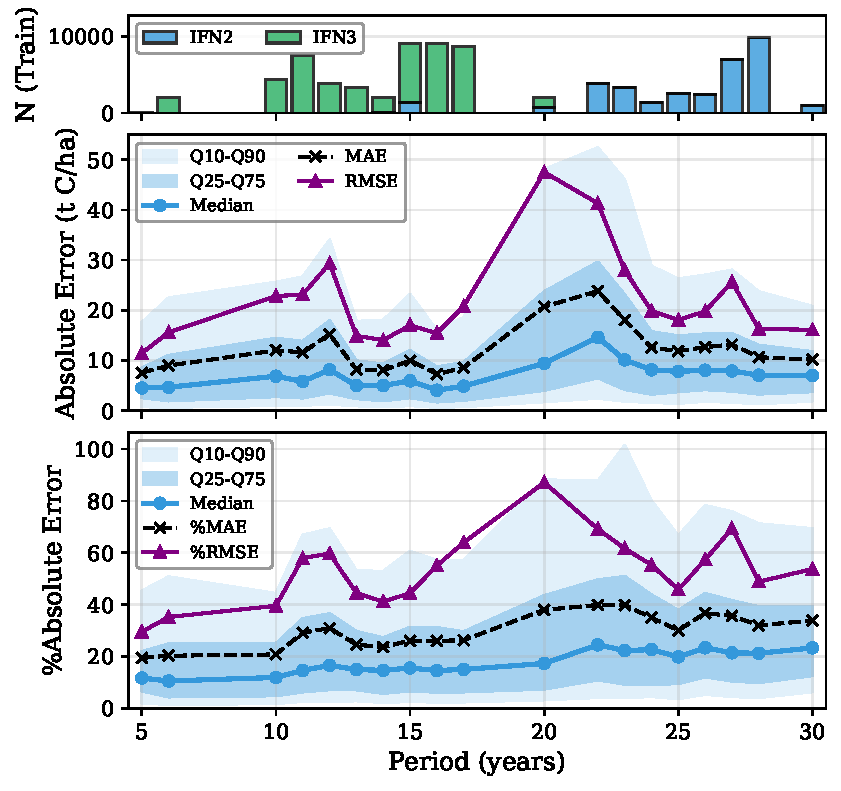
\includegraphics[width=\linewidth]{figuras/09_discusion/c4_LightGBM_metrics.pdf}
        \caption{LightGBM$_{\text{global}}$, \texttt{c4} (tC/ha).}
        \label{fig:LightGBM_rmse_y_pct_rmse_cuantiles}
    \end{subfigure}
    \hfill
    \begin{subfigure}[b]{0.48\linewidth}
        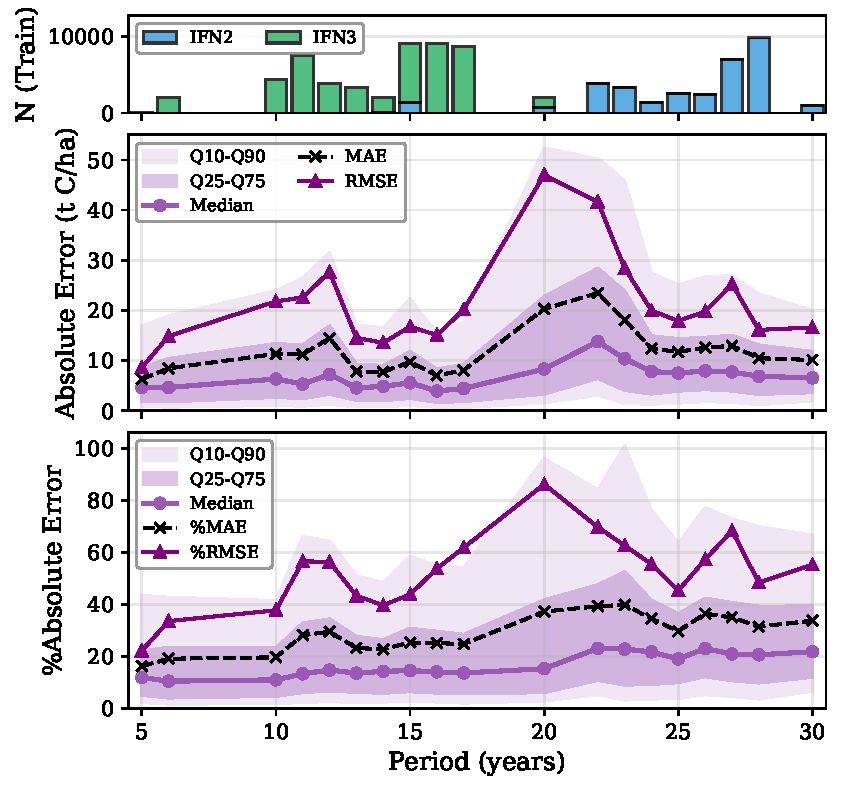
\includegraphics[width=\linewidth]{figuras/09_discusion/c4_Stack5_MLP_metrics.pdf}
        \caption{Global stacking (Conf.~5, MLP), \texttt{c4} (tC/ha).}
        \label{fig:Stack5_MLP_rmse_y_pct_rmse_cuantiles}
    \end{subfigure}
    \\[0.5em]
    \begin{subfigure}[b]{0.48\linewidth}
        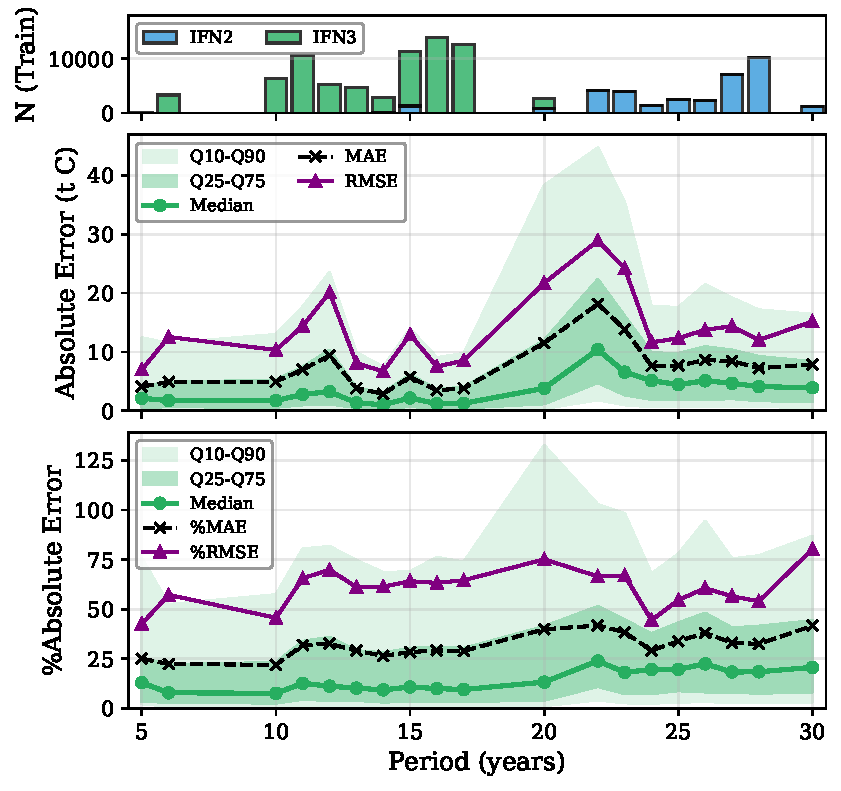
\includegraphics[width=\linewidth]{figuras/09_discusion/carbono_bruto4_CatBoost_metrics.pdf}
        \caption{CatBoost$_{\text{global}}$, \texttt{carbono\_bruto4} (tC).}
        \label{fig:CatBoost_combined}
    \end{subfigure}
    \hfill
    \begin{subfigure}[b]{0.48\linewidth}
        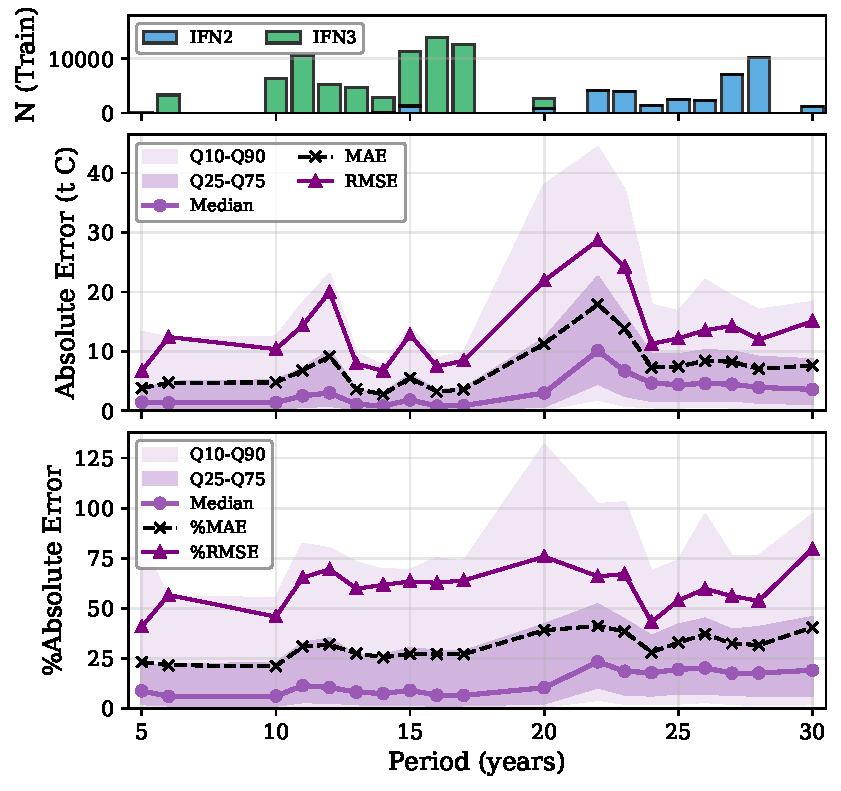
\includegraphics[width=\linewidth]{figuras/09_discusion/carbono_bruto4_Stack5_MLP_metrics.pdf}
        \caption{Global stacking (Conf.~5, MLP), \texttt{carbono\_bruto4} (tC).}
        \label{fig:Stack5_MLP_combined_rmse_y_pct_rmse_cuantiles}
    \end{subfigure}
    \caption{Evolution of absolute error and percentage absolute error in quantiles as a function of the period for the best global models (IFN2$+$IFN3), base and \textit{stacking}, for each target variable.}
    \label{fig:metrics_all}
\end{figure*}

\begin{figure*}[htbp]
    \centering
    \begin{subfigure}[b]{0.48\linewidth}
        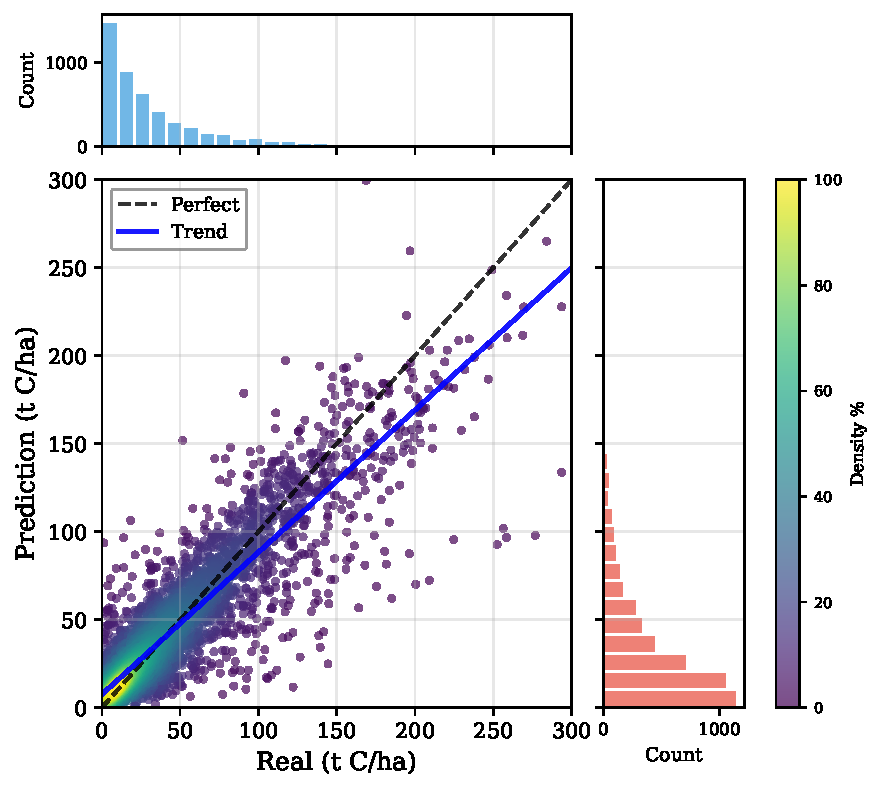
\includegraphics[width=\linewidth]{figuras/09_discusion/c4_LightGBM_density.pdf}
        \caption{LightGBM$_{\text{global}}$, \texttt{c4} (tC/ha).}
        \label{fig:density_LightGBM_0-300}
    \end{subfigure}
    \hfill
    \begin{subfigure}[b]{0.48\linewidth}
        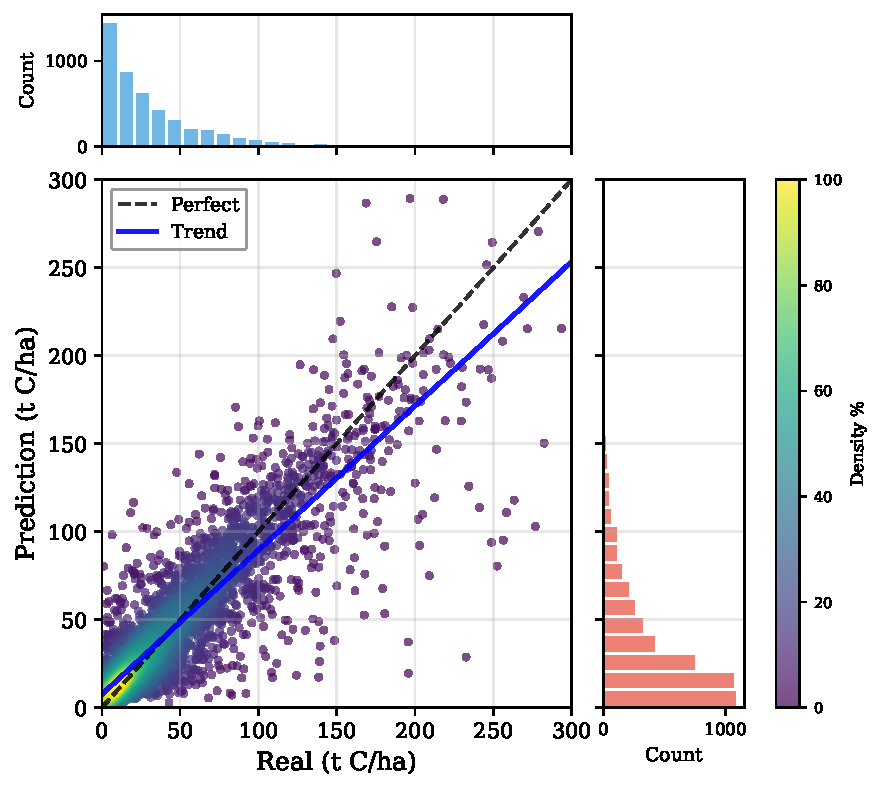
\includegraphics[width=\linewidth]{figuras/09_discusion/c4_Stack5_MLP_density.pdf}
        \caption{Global stacking (Conf.~5, MLP), \texttt{c4} (tC/ha).}
        \label{fig:Stack5_MLP_density}
    \end{subfigure}
    \\[0.5em]
    \begin{subfigure}[b]{0.48\linewidth}
        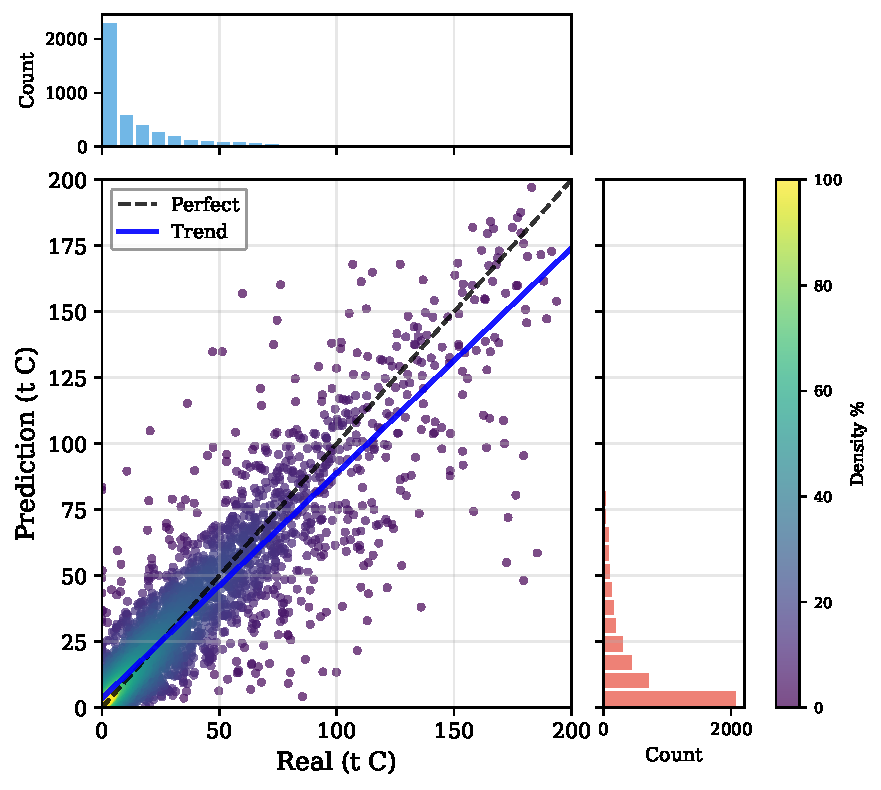
\includegraphics[width=\linewidth]{figuras/09_discusion/carbono_bruto4_CatBoost_density.pdf}
        \caption{CatBoost$_{\text{global}}$, \texttt{carbono\_bruto4} (tC).}
        \label{fig:CatBoost_density}
    \end{subfigure}
    \hfill
    \begin{subfigure}[b]{0.48\linewidth}
        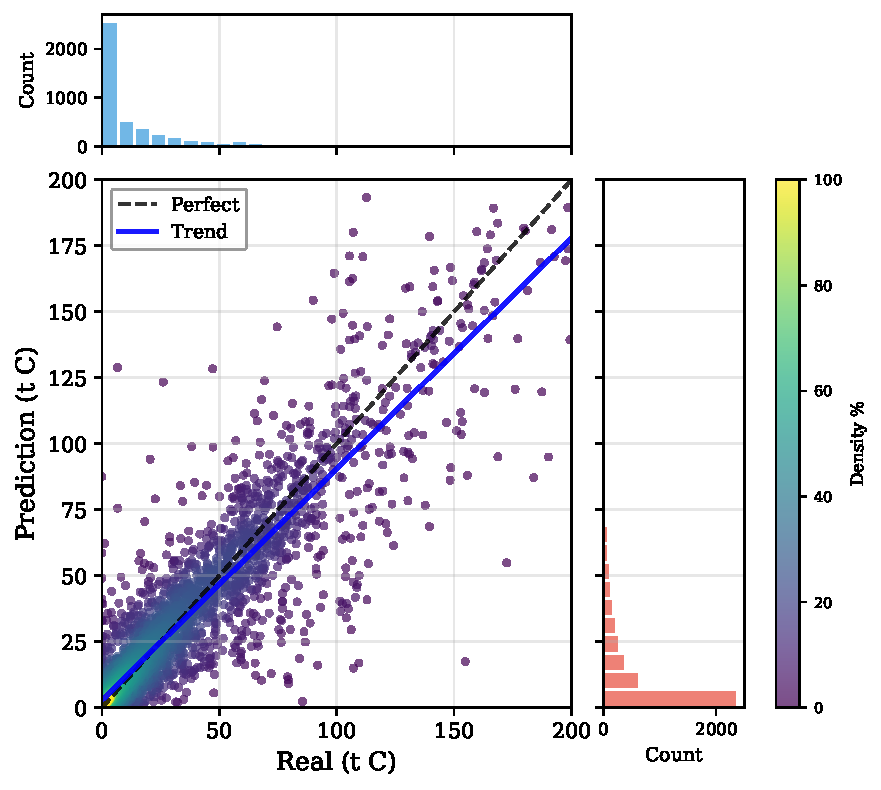
\includegraphics[width=\linewidth]{figuras/09_discusion/carbono_bruto4_Stack5_MLP_density.pdf}
        \caption{Global stacking (Conf.~5, MLP), \texttt{carbono\_bruto4} (tC).}
        \label{fig:Stack5_MLP_density_carbono_bruto4}
    \end{subfigure}
    \caption{Prediction density versus actual values for the best global models (IFN2$+$IFN3), base and \textit{stacking}, for each target variable.}
    \label{fig:density_all}
\end{figure*}

% Tanto en la Figura \ref{fig:LightGBM_rmse_cuantiles} como en la Figura \ref{fig:LightGBM_rmse_porcentual_cuantiles} se observa el mismo comportamiento: las mejores predicciones se obtienen en aquellos casos en los que los datos de entrenamiento provienen del IFN3. Esto se ve claramente en la forma en la que aumentan los errores (sobre todo los del cuantil $90$) cuando se intenta predecir valores para un periodo mayor a $17$ años, valor a partir del cuál los datos del IFN3 se acaban. Observamos que a partir de los $17$ años aumentan en gran medida los valores grandes de error (cuantil $90$) junto con los valores grandes - medios (cuantil $75$). No obstante, los valores medianos y los pequeños - medios (cuantil $25$) se mantienen relativamente estables, aumentando ligeramente con el periodo.

We can observe something we could anticipate: the difficulty of prediction depends on a combination of how far into the future the prediction is desired and the quality and quantity of training data. Starting in the IFN3 range, we can observe that for the first years ($5$, and $6$), despite having few data points, errors are modest. As the period increases (between $10$ and $17$ years), mean and median errors remain relatively stable despite generally having more training data. Large extreme errors (quantile $90$) experience a widespread increase. When we enter the range of years where training data come mainly from the IFN2 (the range between $20$ and $30$ years), although the median and the low-to-medium values (quantile $25$) remain stable, the medium-to-high (quantile $75$) and large (quantile $90$) values increase substantially. This indicates that, even with a large amount of training data (especially for years $27$ and $28$), the combination of lower data quality (always comparing with IFN3) and prediction at distant values makes model prediction harder. Furthermore, as can be seen in Figure \ref{fig:distribucion_variables_combinado}, the values for the first years of IFN2 show high variability, being mostly higher than those of IFN3 for the same years, with greater variability. This, combined with the fact that the amount of data for those years is not excessively large, causes the model to obtain worse predictions.

The fact that median values remain relatively stable across all periods indicates that the model correctly assimilates the behaviour of the target variable both with IFN2 and IFN3 data. On the other hand, the high quantile $90$ errors can be explained by several factors: the high variability of the dataset, the smaller number of field variables collected in the IFN2 (which reduces available information) and the greater inherent difficulty of predicting over long time horizons. This combination makes particular or atypical cases less recognisable by the model, especially when they come from the IFN2, where discriminative capacity is lower than in the IFN3. The aforementioned variability is clearly visible in Figure~\ref{fig:density_LightGBM_0-300}, which shows predicted values versus actual values for the model with the best metrics, along with a distribution histogram.

\paragraph{Stacking models}

The incorporation of \textit{stacking} schemes does not produce substantial, though systematic, increases in the coefficient of determination with respect to the best individual models. Looking at Table \ref{tab:stack_global_c4} we can observe that stacking models present better metrics in the vast majority of cases, always compared with the base models. The best parameters are obtained by the stacking model with configuration 5, which retains all models with competitive performance, together with the neural network meta-model.

The fact that all ensembles improve upon the base models is a sign that this improvement is not a statistical exception, but a real improvement. That is, it is not the case that the metrics are better due to stochasticity in the meta-model parameters, but because the stacking genuinely improves the final result. Obviously, retraining the meta-models with other parameters would change the metrics, but the fact is that the function of improving predictions is indeed achieved with the ensembles. However, the improvement is small, which may mean that depending on the case, simplicity of using one of the base models is preferred over one of the ensembles.

Figure \ref{fig:Stack5_MLP_rmse_y_pct_rmse_cuantiles} shows the evolution of RMSE and percentage RMSE in quantiles for the ensemble model with the best metrics, the stacking with configuration 5 and MLP meta-model. We can observe that the behaviour is practically identical to that of LightGBM, which achieved the best metrics among the base models.
On the other hand, in Figure \ref{fig:Stack5_MLP_density} we can see the scatter plot of predictions versus actual values for the stacking model with configuration 5 and MLP meta-model for the variable \texttt{c4} (tC/ha).


Regarding the structure of the ensembles, the best results are obtained when high-quality, similar-nature base models are combined (mainly \textit{gradient boosting} variants) and meta-models of moderate complexity, such as MLP or linear SVR, are used. In contrast, stacks with few base models or those incorporating excessively flexible meta-models, such as Random Forest at the second level, tend to offer lower performance, probably due to the low dimensionality of the meta-predictor space or unnecessary overfitting of residual noise.



\subsubsection{Variable \texttt{carbono\_bruto4} (in tonnes of carbon)}
\vspace{0.3cm}
\paragraph{Base models}

In the same way as in the previous sections, Figure \ref{fig:CatBoost_combined} shows the evolution of RMSE and \%RMSE in quantiles as a function of the \texttt{periodo} variable for the CatBoost model (the one that achieved the best metrics among the base models) with IFN2 and IFN3 as explanatory variables for the variable in tonnes of carbon, together with the histogram of the distribution of training data as a function of the period variable.


Referring to Figure \ref{fig:CatBoost_combined} we observe the same qualitative behaviour as in the case of the \texttt{c4} variable (with the particularity that units and value range change): the error between quantiles $25$ and $75$ remains at relatively small and constant values, although it is true that it starts smaller and gradually increases as the period variable increases. Extreme errors (quantile $90$) remain high. In fact, looking at the highest values of the percentage RMSE for quantile $90$, we observe that notably higher values are reached than in the case of the \texttt{c4} variable, reaching up to $130\%$ when for \texttt{c4} it barely exceeded $100\%$ for the worst case. This is noteworthy, since the global metrics for predictions of the variable \texttt{carbono\_bruto4} (see Table \ref{tab:base_global_carbono_bruto4}) are systematically better than those of the variable \texttt{c4} (see Table \ref{tab:base_global_c4}). That is, the variable \texttt{carbono\_bruto4} (tonnes) is generally easier for models to predict than the variable \texttt{c4} (tonnes per hectare), but the opposite occurs in particular cases, where the highest errors shoot up in a more exaggerated manner than in the same case for the \texttt{c4} variable. The increase in error when moving from the IFN2 to IFN3 year range is also observed, caused by the increase in variability of the second inventory data (see Figure \ref{fig:distribucion_variables_combinado}).

As in the previous sections, Figure \ref{fig:CatBoost_density} shows a scatter plot of predictions versus actual values for the CatBoost model for the case under consideration.




\paragraph{Stacking models}

The results obtained in this section are very similar to those obtained with the stacking models for the \texttt{c4} (tC/ha) variable. That is, we find a systematic improvement in all stacking models over the base models, but that improvement is small. This causes the results to be strictly better, as can be seen in Table \ref{tab:stack_global_carbono_bruto4} compared with the base model metrics in Table \ref{tab:base_global_carbono_bruto4}. Again, the fact that the improvement of stacking models over base models is systematic indicates that we are not facing a statistical incident, but rather that the stacking format is capable of improving predictions by choosing the best decisions from each model. However, as noted above, the complexity of training five models in addition to the meta-model may be inconvenient compared to the possibility of using, for example, the best of the individual models.

The ensemble model that provides the best metrics for predicting the \texttt{carbono\_bruto4} (tC) variable is configuration 5 with an MLP meta-model, as was also the case for the \texttt{c4} (tC/ha) variable. The evolution of RMSE and percentage RMSE in quantiles as a function of the \texttt{periodo} variable for this model can be visualised in Figure \ref{fig:Stack5_MLP_combined_rmse_y_pct_rmse_cuantiles}.



On the other hand, Figure \ref{fig:Stack5_MLP_density_carbono_bruto4} shows a scatter plot of predictions versus actual values for the stacking model with configuration 5, MLP meta-model and the variable \texttt{carbono\_bruto4} (tC).

\subsection{Individual models trained on IFN2 or IFN3 only.}

When comparing the performance of ``global'' models (trained on the combined IFN2 and IFN3 dataset) versus ``local'' models (trained exclusively on IFN2 or IFN3), differentiated behaviour is observed depending on the test inventory. For IFN3, local models outperform global ones in terms of accuracy metrics. Conversely, for IFN2, global models show superior performance.

A possible explanation for this phenomenon lies in the quality and quantity of information contained in each inventory. The IFN2 data, being less informative or having fewer variables, appear to benefit from joint learning with IFN3 data, allowing models to capture additional patterns and improve their generalisation capacity on the second inventory. In contrast, for IFN3, whose data possess higher intrinsic quality, the inclusion of IFN2 records during training could be introducing noise or unwanted variability, which ultimately penalises the accuracy of the final model predictions on this dataset.

\begin{figure*}[htbp]
    \centering
    \begin{subfigure}[b]{0.48\linewidth}
        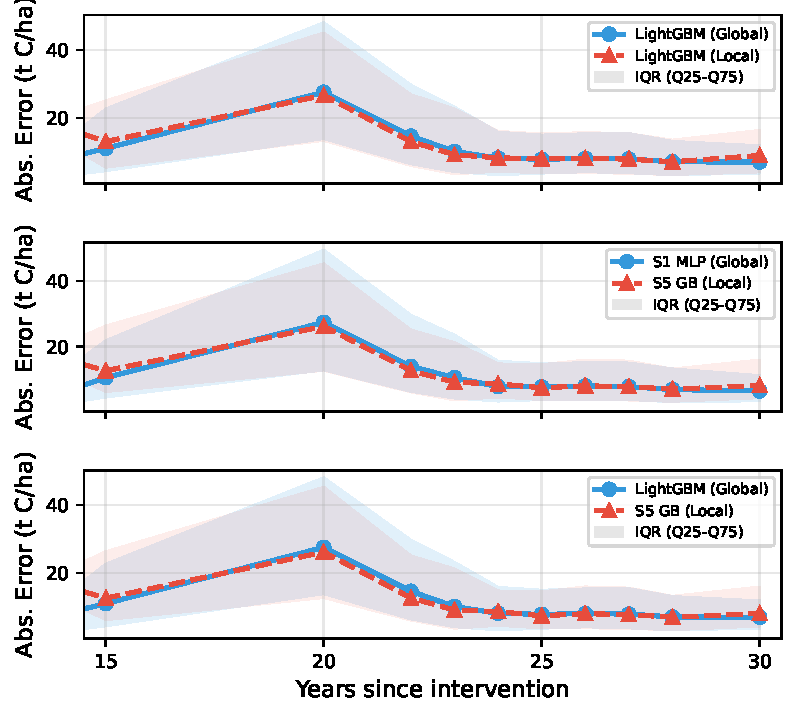
\includegraphics[width=\linewidth]{figuras/09_discusion/Consolidado_IFN2_c4_clean.pdf}
        \caption{IFN2, \texttt{c4} (tC/ha).}
        \label{fig:comparativa_mejores}
    \end{subfigure}
    \hfill
    \begin{subfigure}[b]{0.48\linewidth}
        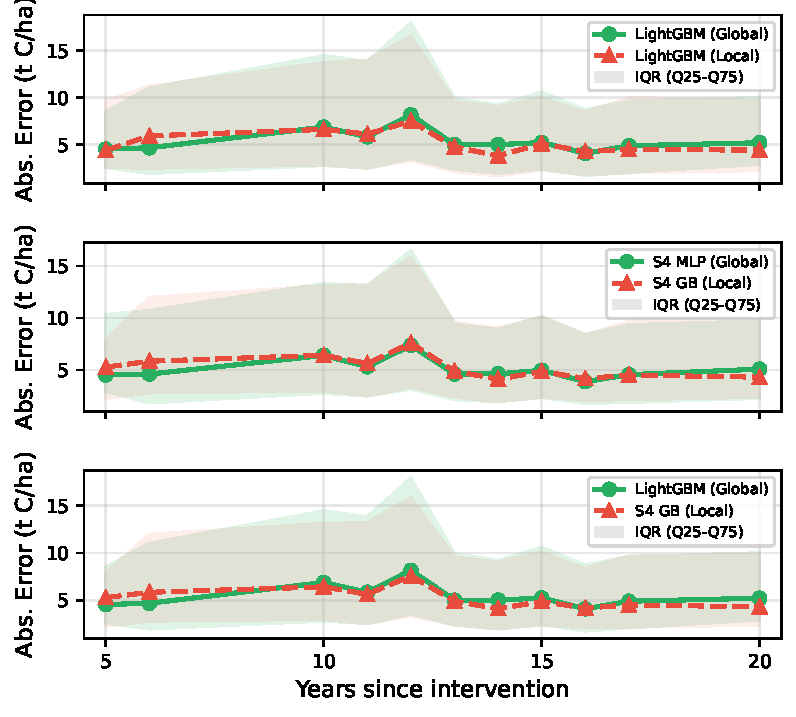
\includegraphics[width=\linewidth]{figuras/09_discusion/Consolidado_IFN3_c4_clean.pdf}
        \caption{IFN3, \texttt{c4} (tC/ha).}
        \label{fig:disc_sub2}
    \end{subfigure}
    \\[0.5em]
    \begin{subfigure}[b]{0.48\linewidth}
        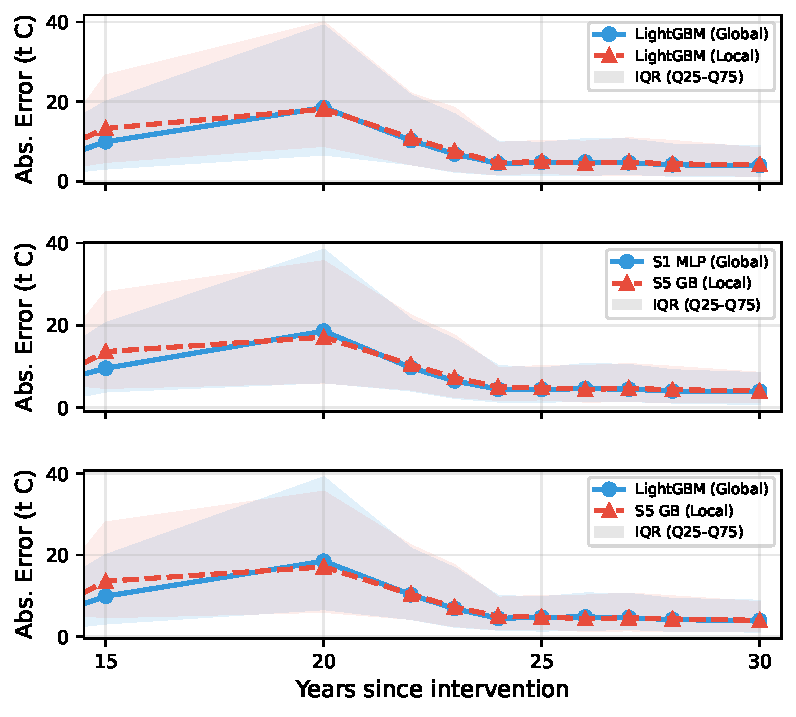
\includegraphics[width=\linewidth]{figuras/09_discusion/Consolidado_IFN2_carbono_bruto4_clean.pdf}
        \caption{IFN2, \texttt{carbono\_bruto4} (tC).}
        \label{fig:disc_sub3}
    \end{subfigure}
    \hfill
    \begin{subfigure}[b]{0.48\linewidth}
        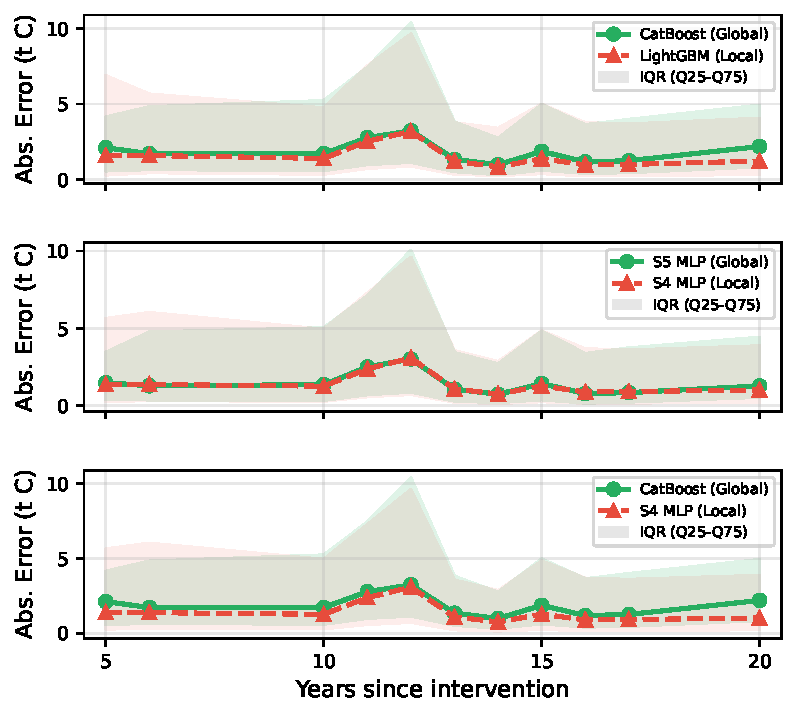
\includegraphics[width=\linewidth]{figuras/09_discusion/Consolidado_IFN3_carbono_bruto4_clean.pdf}
        \caption{IFN3, \texttt{carbono\_bruto4} (tC).}
        \label{fig:disc_sub4}
    \end{subfigure}
    \caption{Comparison of absolute error by inventory and target variable: best global vs.\ local base models, global vs.\ local stacking models, and best base model vs.\ best stacking model.}
    \label{fig:consolidado_all}
\end{figure*}

Figure \ref{fig:comparativa_mejores} shows a comparison between the best global vs.\ local base models (top), best global vs.\ local stacking models (middle) and best base model vs.\ best stacking model (bottom). We observe that in general the lower errors for IFN2 are committed by the global models, while for IFN3 it is the local models that do the better job.


% \subsubsection{Comportamiento global de los modelos}

\subsubsection{Assimilation of target variable behaviour}

With the metrics we have set out and the analysis carried out in this section, it seems clear that, while the results are far from perfect, the models are capable of understanding the logic and meaning of each variable to obtain a prediction with a degree of accuracy that depends on the nature of the instance in question. Another test we can perform to check whether the model results are logical is the one shown in Figures \ref{fig:sensibilidad_escenarios} and \ref{fig:sensibilidad_escenarios_carbono_bruto4}.
These figures show the evolution of several particular cases as time progresses between measurement and prediction. The selected cases are real within the available data. They were selected with the aim of showing how the models behave for more or less common initial carbon configurations. To this end, for each data instance, the \texttt{npies_x} variables were summed, and then the values closest to percentiles 10, 35, 65 and 90 for the resulting variable were selected. This avoids potential problems arising from selecting unrealistic examples.


\begin{figure}
      \centering
      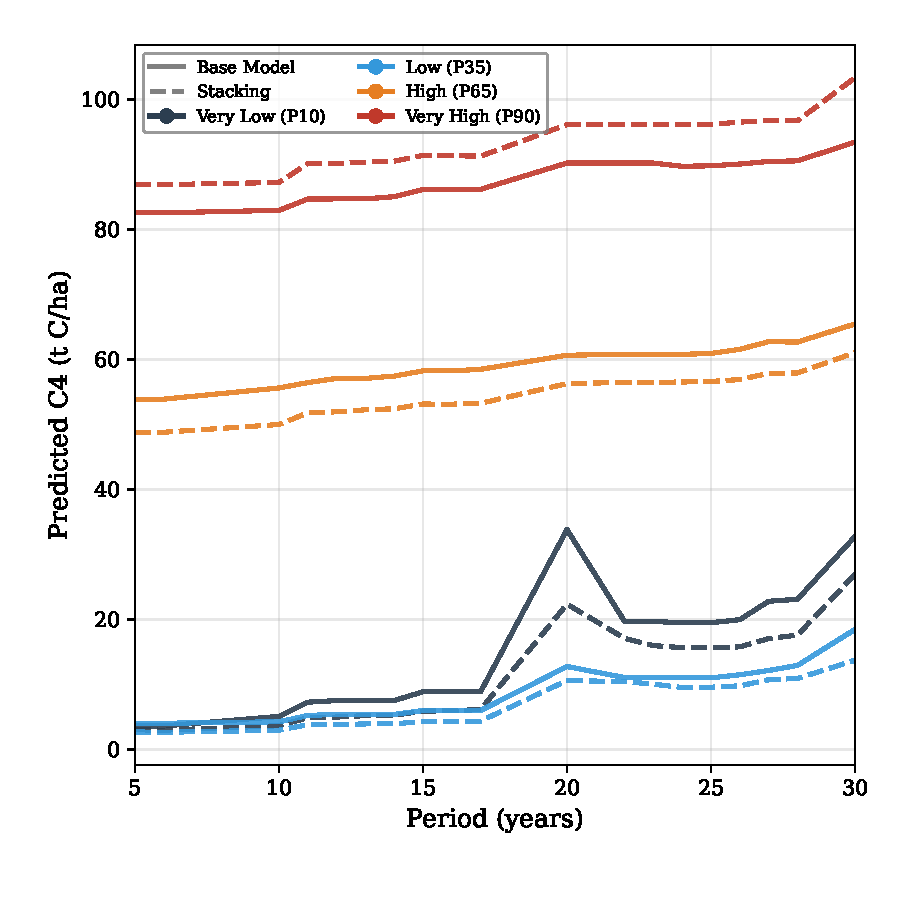
\includegraphics[width=\linewidth]{figuras/09_discusion/sensibilidad_escenarios_c4_P10_P35_P65_P90.pdf}
      \caption{Evolution of the amount of carbon in tonnes per hectare (\texttt{c4}) for several scenarios.}
      \label{fig:sensibilidad_escenarios}
\end{figure}

\begin{figure}
      \centering
      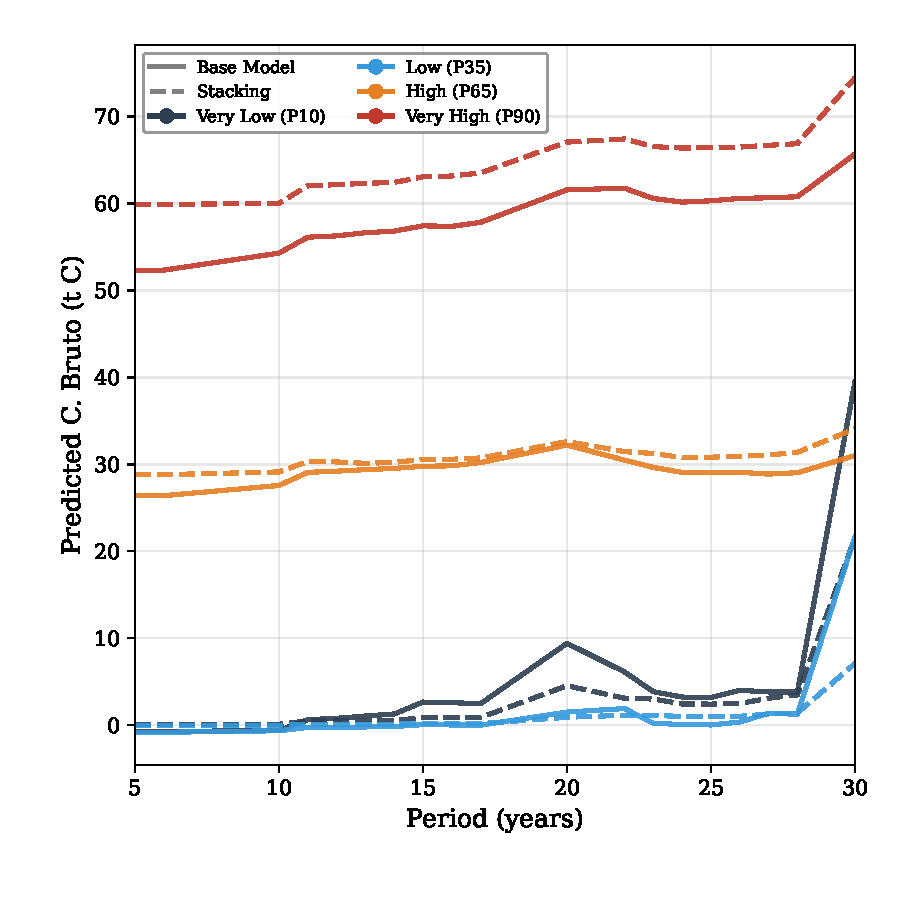
\includegraphics[width=\linewidth]{figuras/09_discusion/sensibilidad_escenarios_carbono_bruto4_P10_P35_P65_P90.pdf}
      \caption{Evolution of the amount of carbon in tonnes (\texttt{carbono\_bruto4}) for several scenarios.}
      \label{fig:sensibilidad_escenarios_carbono_bruto4}
\end{figure}

We can highlight the following features:
\begin{itemize}
      \item The lines of the base models and ensembles for each case are very close together, which is consistent with the obtained metrics, which were very similar to each other.
      \item The general trend is upward, i.e., the models correctly capture the behaviour of tree growth over time for the studied years.
      \item In year $17$ there is a widespread abrupt increase, which is more exaggerated the smaller the percentile of the case study. This is easy to understand by looking at the data, since the values of the variable to be predicted experience a generalised increase when moving from the IFN2 years to those of the IFN3, as can be seen in Figure \ref{fig:distribucion_variables_combinado}. This change (where the model begins to ingest IFN2 data instead of IFN3 data) occurs mainly in year $17$. This can be seen in the histogram of Figure \ref{fig:Stack5_MLP_combined_rmse_y_pct_rmse_cuantiles}, for example. The reason why the jump occurs at small percentiles is that these small values in the IFN2 data barely exist or are less common. The model has seen that for those years carbon values are, in general, higher, and that is what it predicts. In fact, Figure \ref{fig:distribucion_variables_combinado} shows that for the initial years of the IFN2 data, carbon values increase and then decrease, and this is exactly what we see in the predictions: an increase followed by a decrease.
      \item We can also see an abrupt increase in many cases when moving from year $29$ to $30$, especially in the case of the variable in tonnes of raw carbon (Figure \ref{fig:sensibilidad_escenarios_carbono_bruto4}). These years coincide with a scarcity of data, as can be seen in the histogram of Figure \ref{fig:distribucion_variables_combinado}. It is to be expected that predictions for those years will be less reliable, especially for an extreme value.
\end{itemize}


\subsubsection{Model performance as a function of the target variable value}

If we analyse the global metrics in the tables of Section \ref{sec:resultados}, we notice that RMSE values are notably larger than MAE values, specifically around twice as large in most cases. Because RMSE penalises large errors much more heavily than MAE, this is indicative of the presence of outliers in the error. We have already seen throughout this section that the largest errors occur in the range of years in which the IFN2 is the main data source, as can be seen in Figures \ref{fig:LightGBM_rmse_y_pct_rmse_cuantiles}, \ref{fig:Stack5_MLP_rmse_y_pct_rmse_cuantiles}, \ref{fig:CatBoost_combined} and \ref{fig:Stack5_MLP_combined_rmse_y_pct_rmse_cuantiles}, and the main conclusion is that the quality or quantity of information contained in this inventory is inferior. However, this does not fully answer the question of in which cases the model predicts best, beyond the obvious fact that prediction will be better the closer in time and the more data available for that year. This is why Figures \ref{fig:SMAPE_RMSE_deciles_c4_carbono_bruto4} and \ref{fig:distribucion_carbono_bruto4_combinado} can be useful. These figures show the distribution of errors, specifically RMSE and SMAPE, as a function of the target variable for \texttt{c4} and \texttt{carbono\_bruto4} respectively, in deciles for the base models.

\begin{figure}
      \centering
      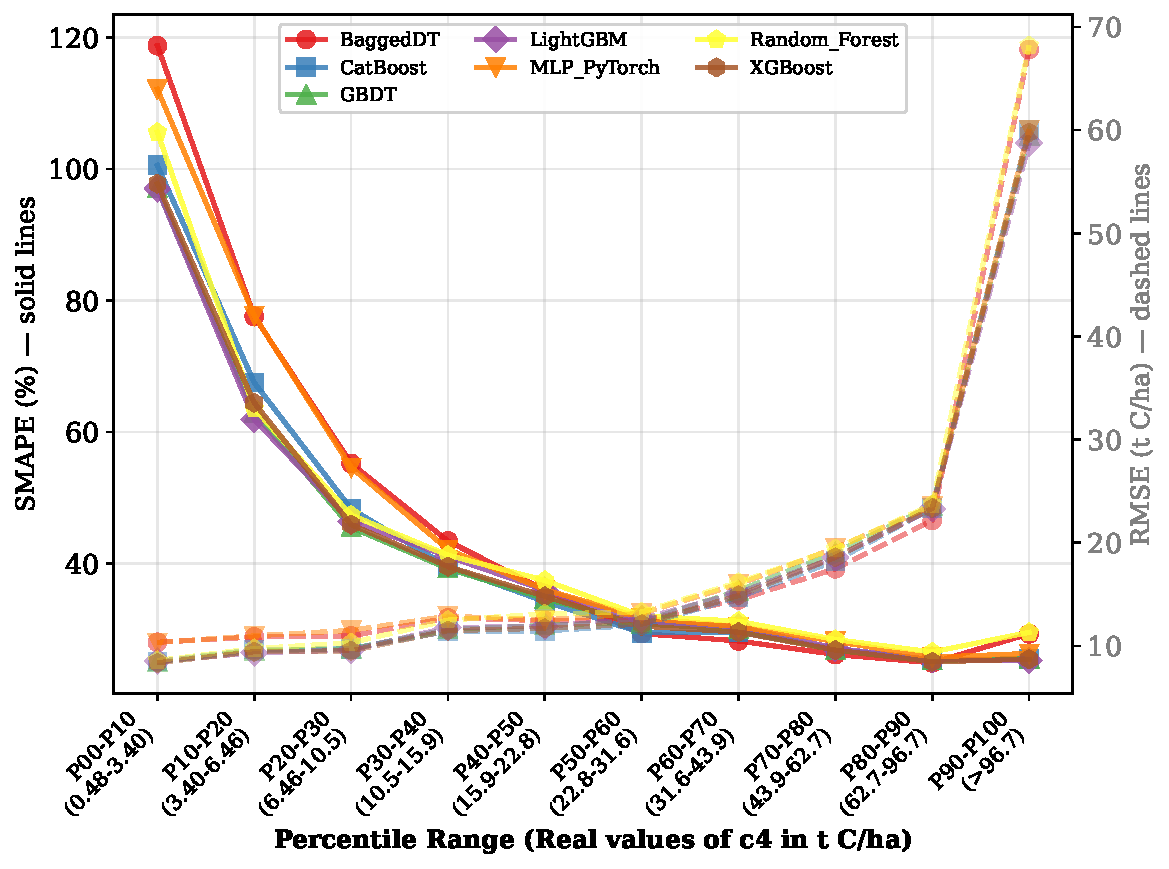
\includegraphics[width=\linewidth]{figuras/09_discusion/c4_base_models_SMAPE_RMSE_percentiles.pdf}
      \caption{Distribution of SMAPE and RMSE as a function of the target variable for \texttt{c4} in deciles.}
      \label{fig:SMAPE_RMSE_deciles_c4_carbono_bruto4}
\end{figure}

\begin{figure}
      \centering
      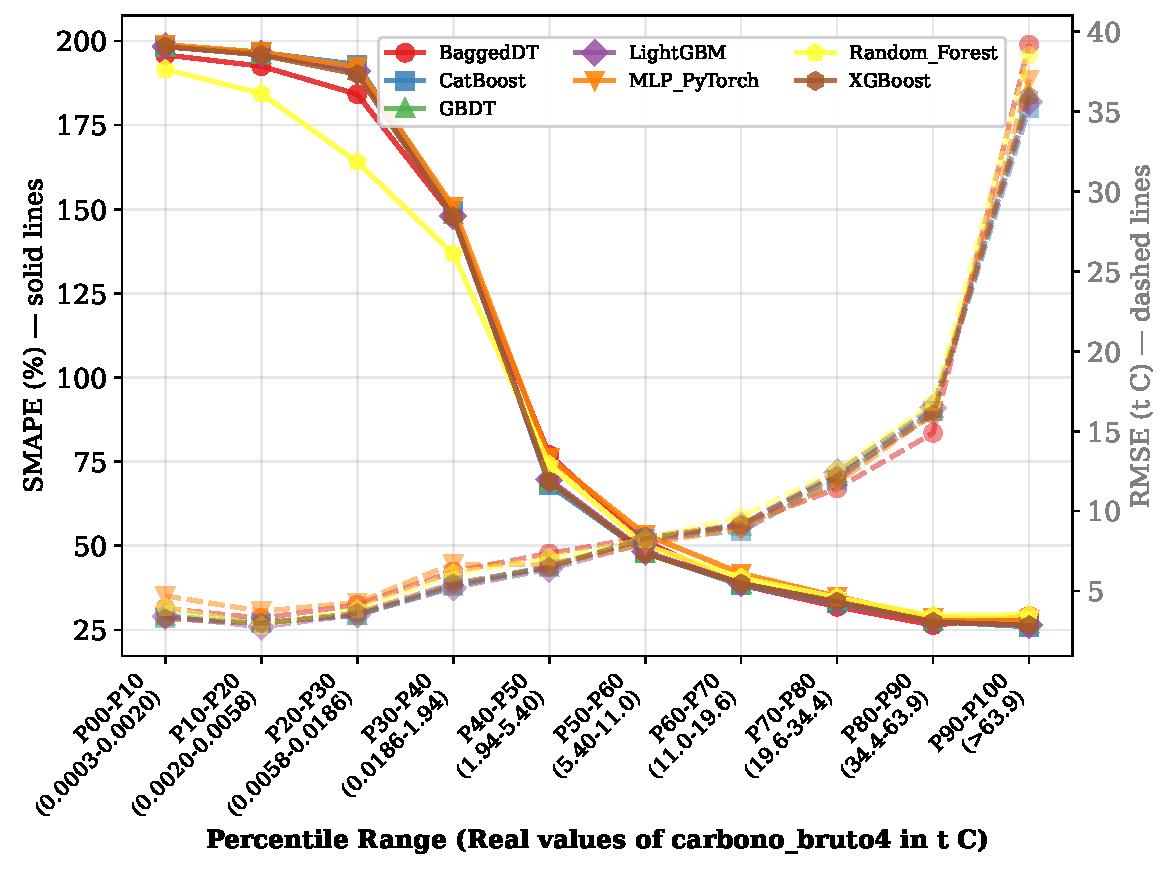
\includegraphics[width=\linewidth]{figuras/09_discusion/carbono_bruto4_base_models_SMAPE_RMSE_percentiles.pdf}
      \caption{Distribution of SMAPE and RMSE as a function of the target variable for \texttt{carbono\_bruto4} in deciles.}
      \label{fig:distribucion_carbono_bruto4_combinado}
\end{figure}


We quickly notice the following: predictions for small values of the target carbon (first deciles) are poor (large SMAPE) despite having the smallest absolute error (small RMSE). Then, as the target carbon increases, RMSE increases slightly while SMAPE decreases much more rapidly, reaching values close to $25\%$. In both cases the best results are achieved when the target carbon is larger, despite a significant increase in RMSE between the second-to-last and last decile. Since this occurs for all models, it suggests that prediction difficulty is not homogeneous across all situations or amounts of carbon, and that despite the lowest-carbon percentiles having the smallest RMSE, model accuracy is not sufficient to make a decent prediction in situations with little biomass. This was predictable, since a larger absolute error for a larger forest plot does not necessarily imply a worse relative error.

Also noteworthy is the fact that the initial deciles have very close carbon ranges, especially for the \texttt{carbono\_bruto4} variable, where the first decile ranges from $0.0003$~tC to $0.0020$~tC. This large number of values with such small carbon does not help models obtain a good prediction. The higher densities at small carbon values are clearly visible in Figures \ref{fig:density_LightGBM_0-300}, \ref{fig:Stack5_MLP_density}, \ref{fig:CatBoost_density} and \ref{fig:Stack5_MLP_density_carbono_bruto4}.

\subsection{Model interpretability: SHAP analysis}
\label{sec:interpretabilidad_shap}

Thanks to the SHAP value analysis we can add explainability to the models, finding out which variables the model gives more importance to and in which cases these values cause the carbon prediction to be higher or lower. In Table \ref{tab:shap_rank_abs} we can observe the mean importance rank of variables with the highest absolute SHAP value, both averaged across all cases (first column ``Mean'') and by source inventory and target variable. In this table we see that the most consistently important variables are \texttt{npies}, \texttt{especie\_id}, \texttt{ocupa} and \texttt{radio}, i.e., variables purely related to the forest structure. The rest of the variables in the table have more variability across the different configurations, where meteorological variables (which appear to be more important than the climatic variable we added, the Martonne index) and edaphic variables are mainly interleaved.

% ============================================================
% Tabla: Ranking medio de variables por |SHAP|
% ============================================================
\begin{table*}[htbp]
  \centering
  \footnotesize
  \caption{Mean SHAP rank per variable across LightGBM, XGBoost, CatBoost, GBDT and MLP (n=2000 samples; rank 1 = most important).}
  \label{tab:shap_rank_abs}
  \begin{tabular}{lccccccc}
    \toprule
    Variable & \textbf{Mean} & \makecell{\textbf{IFN2} \\ \textbf{c4}} & \makecell{\textbf{IFN2} \\ \textbf{carbono\_b4}} & \makecell{\textbf{IFN3} \\ \textbf{c4}} & \makecell{\textbf{IFN3} \\ \textbf{carbono\_b4}} & \makecell{\textbf{IFN2+3} \\ \textbf{c4}} & \makecell{\textbf{IFN2+3} \\ \textbf{carbono\_b4}} \\
    \midrule
    npies* (Density) & \textbf{1} & \textbf{1} & \textbf{1} & \textbf{1} & \textbf{1} & \textbf{1} & \textbf{1} \\
    especie\_id* & 2.2 & 2 & 2 & 2.2 & 2.8 & 2.2 & 2.2 \\
    ocupa & 2.9 & 3.2 & 3 & 3 & 2.2 & 2.8 & 3 \\
    radio & 4.2 & 4.2 & 4.2 & 4.2 & 4.2 & 4.2 & 4.4 \\
    gndvi\_mean\_verano & 6.5 & 5.6 & 5 & 7 & 7 & 8 & 6.6 \\
    tipo\_especie* & 7.1 & 11.6 & 8.8 & 4.6 & 5.8 & 6 & 6 \\
    periodo\_agrupado & 8.4 & 13 & 8 & 10.6 & 8.6 & 5.2 & 5 \\
    skt\_mean\_verano & 9.6 & 6.8 & --- & 10.4 & --- & 11.6 & --- \\
    rocosidad\_id* & 11 & 9 & 7.6 & 17.2 & 12 & 10.2 & 9.8 \\
    fccarb & 11.4 & --- & --- & 9 & 10 & 14 & 12.6 \\
    evi\_mean\_primavera & 11.8 & 12 & 10.6 & 13.6 & 11.2 & 13.2 & 10.4 \\
    elevacion & 12.6 & 12.6 & 7.4 & 15.8 & 12.8 & 14.4 & 12.4 \\
    tratmasa\_id* & 13.2 & --- & --- & 8 & 7.2 & 18.8 & 18.8 \\
    estado\_id* & 13.5 & 21.8 & 12.8 & 17.2 & 12.6 & 8.8 & 8 \\
    ndii\_mean\_primavera & 14.5 & 17 & 11.6 & 14.2 & 15.6 & 15.4 & 13.4 \\
    skt\_mean\_primavera & 15.1 & 17.4 & --- & 13.4 & --- & 14.6 & --- \\
    pr\_sum\_otoño & 15.7 & 16.4 & --- & 14.4 & --- & 16.4 & --- \\
    pr\_sum\_primavera & 15.7 & 10.6 & --- & 17.6 & --- & 19 & --- \\
    pr\_sum\_invierno & 16 & 8.6 & --- & 21.8 & --- & 17.6 & --- \\
    martonneidx\_id* & 16.4 & 18.2 & 10.2 & 24.2 & 13.4 & 20.6 & 11.8 \\
    skt\_std\_verano & 18.4 & 13.2 & --- & 22.8 & --- & 19.2 & --- \\
    skt\_std\_primavera & 18.4 & 15.8 & --- & 20 & --- & 19.4 & --- \\
    orientacion\_cat* & 18.9 & 19.8 & 14.4 & 23 & 17 & 21.4 & 18 \\
    modcomb\_id* & 18.9 & --- & --- & 18.8 & 14 & 26 & 16.8 \\
    gndvi\_std\_primavera & 19.8 & 20.8 & 14.6 & 24 & 18 & 24.8 & 16.6 \\
    pendiente\_cat* & 20 & 20.4 & 15.4 & 26.2 & 18 & 23.8 & 16.4 \\
    pr\_sum\_verano & 20.3 & 19.4 & --- & 21.2 & --- & 20.4 & --- \\
    nivel2\_id* & 20.6 & --- & --- & 20.6 & 17.2 & 27 & 17.6 \\
    disesp\_id* & 23.3 & 24.6 & 16.4 & 29 & 20.4 & 29 & 20.2 \\
    \bottomrule
  \end{tabular}
\end{table*}

The meteorological variable that consistently has the most importance according to our analysis is the mean value of the GNDVI index in summer (\texttt{gndvi_mean_verano}), which stands out both by position and consistency. This is expected, since it is in summer when forest vegetation has the greatest vigour, and the GNDVI index is a more useful indicator in this season compared to others such as NDVI, as it does not have saturation problems in dense canopies \cite{eos2025indices_vegetacion, ign_pnoa_lidar_tercera}. Furthermore, this index serves to estimate photosynthetic activity, a variable directly related to both the amount and health of vegetation.

In Figures \ref{fig:SHAP_LightGBM_IFN2_c4}, \ref{fig:SHAP_LightGBM_IFN3_c4} and \ref{fig:SHAP_LightGBM_IFN2_3_c4} we can see a comparison between the SHAP variables of the different configurations for the LightGBM model and the target variable \texttt{c4}. It should be noted that for the two most important variables for the analysis (\texttt{npies}, \texttt{especie\_id} and \texttt{ocupa}), the x-axis scale is different from the rest, as their SHAP value is notably larger. This was done to facilitate visualisation. The variables whose text is coloured are categorical variables (also marked with an asterisk, *), and their colour indicates the treatment applied for inclusion in the figure. First, there is \texttt{npies}. This variable actually consists of several, one for each diameter class (\texttt{npies\_5}, \texttt{npies\_10}, \texttt{npies\_15}, etc.). The green text colour indicates that for each diameter class the analysis was performed individually and then all classes were combined in the same row of the plot. That is, when the colour of the point indicates that the variable value is ``high'', this is normalised to each diameter class, since a high value of the variable \texttt{npies\_5} is not comparable with a high value of \texttt{npies\_70}. The purple text colour indicates that the categorical variable is purely nominal, i.e., it has no order despite being passed to the model encoded in numerical format. This occurs with the variable \texttt{especie\_id}, where a higher numerical value does not indicate, for example, a higher carbon absorption. In this case, the colour of each point expresses the mean of the target variable for each species, so that all points of the same species will have the same colour. This often produces an obvious result: species that absorb more carbon will be those with a higher SHAP value, and therefore will be located generally to the right (which is indeed the case). However, it is the only way found to include this variable in the figure, since it had to be present due to its high importance for the model. If the text colour is orange, it means the categorical variable is ordinal. That is, the category follows an order that makes sense to represent by colours. For example, the variable \texttt{rocosidad\_id} goes from value $1$, ``no stoniness'', to $5$, ``rocky'', with the increase in the variable related to an increase in the indicated characteristic. Finally, black text colour indicates that the variable is continuous and is treated as expected.

\begin{figure}
      \centering
      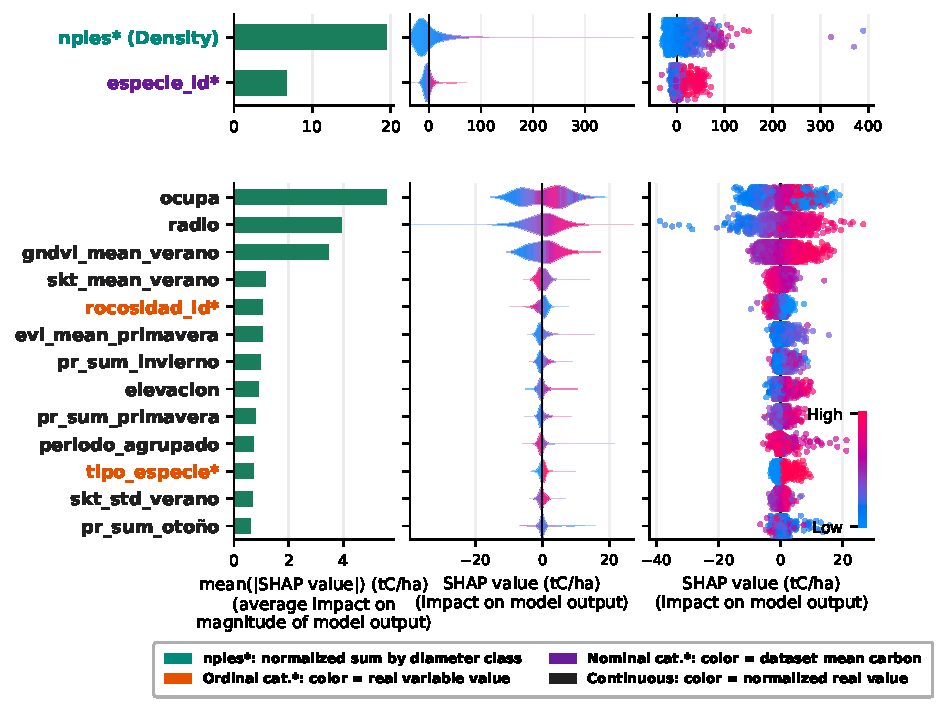
\includegraphics[width=\linewidth]{figuras/09_discusion/shap_summary_LightGBM_local_n2000_ifn2.pdf}
      \caption{SHAP analysis for the LightGBM model trained on IFN2 data with target variable \texttt{c4} (tC/ha).}
      \label{fig:SHAP_LightGBM_IFN2_c4}
\end{figure}

\begin{figure}
      \centering
      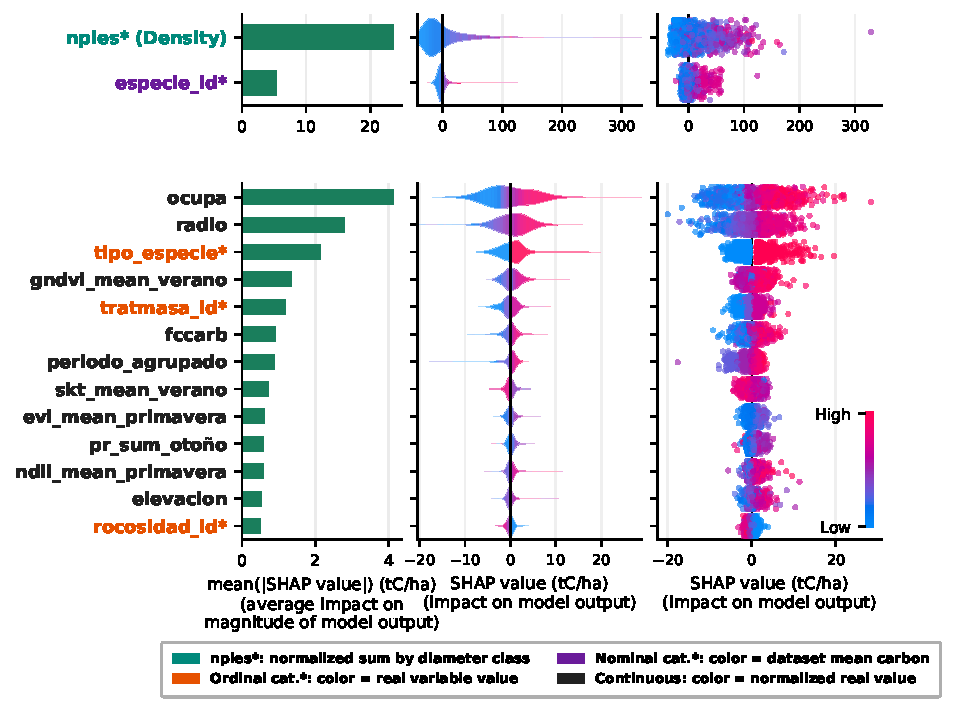
\includegraphics[width=\linewidth]{figuras/09_discusion/shap_summary_LightGBM_local_n2000_ifn3.pdf}
      \caption{SHAP analysis for the LightGBM model trained on IFN3 data with target variable \texttt{c4} (tC/ha).}
      \label{fig:SHAP_LightGBM_IFN3_c4}
\end{figure}

\begin{figure}
      \centering
      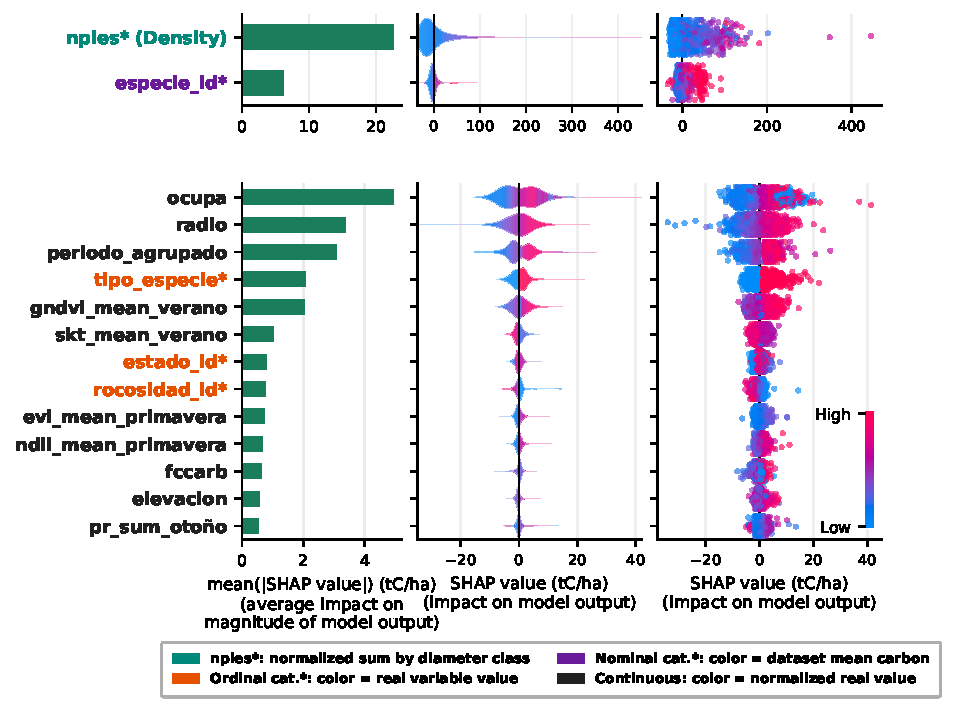
\includegraphics[width=\linewidth]{figuras/09_discusion/shap_summary_LightGBM_global_n2000_ifn23.pdf}
      \caption{SHAP analysis for the LightGBM model trained on IFN2 and IFN3 data with target variable \texttt{c4} (tC/ha).}
      \label{fig:SHAP_LightGBM_IFN2_3_c4}
\end{figure}


In Figures \ref{fig:SHAP_LightGBM_IFN2_c4}, \ref{fig:SHAP_LightGBM_IFN3_c4} and \ref{fig:SHAP_LightGBM_IFN2_3_c4} we see that the two most important variables are always \texttt{npies} and \texttt{especie\_id}, as we had seen in Table \ref{tab:shap_rank_abs}. The remaining variables change order depending on the case, but speaking of the whole set, the variables identified as important tend to be common across the three cases in the Figures. It should be noted that, although the positions of the variables do not exactly match between the case of the model trained solely with IFN2 data (Figure \ref{fig:SHAP_LightGBM_IFN2_c4}) and the model trained with IFN2 and IFN3 data (Figure \ref{fig:SHAP_LightGBM_IFN2_3_c4}), the variables present in the top $15$ shown are practically the same in total (except for \texttt{tratmasa\_id}) and \texttt{estado\_id} which are swapped. Variables exclusive to IFN3, such as \texttt{tratmasa\_id}, also appear, indicating that these new variables incorporated into successive inventories provide useful information for the study of forests, and specifically for studying carbon capture.

Looking at the values in Figures \ref{fig:SHAP_LightGBM_IFN2_c4}, \ref{fig:SHAP_LightGBM_IFN3_c4} and \ref{fig:SHAP_LightGBM_IFN2_3_c4} we can highlight some interesting results that support the idea that the model has correctly incorporated the information:
\begin{itemize}
      \item Looking at the variable \texttt{npies}, we observe that a higher number of initial trees corresponds to a higher SHAP value, i.e., more carbon.
      \item As stated earlier, for the variable \texttt{gndvi\_mean\_verano} a higher SHAP index is obtained for cases where its value is also higher. This is logical, since the GNDVI index measures photosynthetic activity. A higher value of this index corresponds to a greater presence of active vegetation, and therefore greater carbon capture.
      \item The variable \texttt{periodo\_agrupado} indicates the number of years between the measurement and the moment at which we wish to make the estimate, so it is expected that a higher value corresponds to a higher SHAP value, i.e., more carbon. This is what we find for the IFN3 case (Figure \ref{fig:SHAP_LightGBM_IFN3_c4}) and IFN2 and 3 (Figure \ref{fig:SHAP_LightGBM_IFN2_3_c4}). Curiously, for the IFN2 case (Figure \ref{fig:SHAP_LightGBM_IFN2_c4}) this relationship is less clear, which also coincides with the SHAP model assigning it relatively lower importance.
      \item The variable \texttt{tipo\_especie} has a very clear distinction in all cases. This is a binary variable in which value $0$ corresponds to conifers and value $1$ corresponds to broadleaves. According to the analysis, broadleaf species obtain on average a higher SHAP index, i.e., a greater amount of carbon associated with them. This is consistent with the literature, and specifically with studies carried out using the Spanish National Forest Inventory, which quantify the mean carbon \textit{stock} in broadleaf stands at $48.5 \pm 0.3$~Mg/ha compared to $41.8 \pm 0.2$~Mg/ha in conifers for mainland Spain \cite{vayreda2012carbon}.

      For further detail, Figure \ref{fig:SHAP_species_LightGBM_global} presents a breakdown of the SHAP index by species for the LightGBM model trained on data from both inventories and with \texttt{c4} as the target variable. It can be observed that broadleaves occupy almost all the positions in which carbon increases, with \textit{Eucalyptus globulus} as the first species, a species that has been causing controversy in northern Spain for years due to its possible characterisation as an invasive species \cite{miteco2017eucalyptus,greenpeace2025eucalipto}. However, it should be noted that this result reflects the biomass inventoried in the IFN, and does not imply that eucalyptus is the most appropriate option from a sustainable forest management perspective, given its high water consumption, its association with a higher fire risk, the loss of biodiversity it can cause, the difficulty of eradication, or the danger associated with the involuntary introduction of associated species, such as insects or fungi, displacing other native species \cite{miteco2017eucalyptus, cordero1999gonipterus, diez2005mycorrhizal}.
\end{itemize}

\begin{figure}
      \centering
      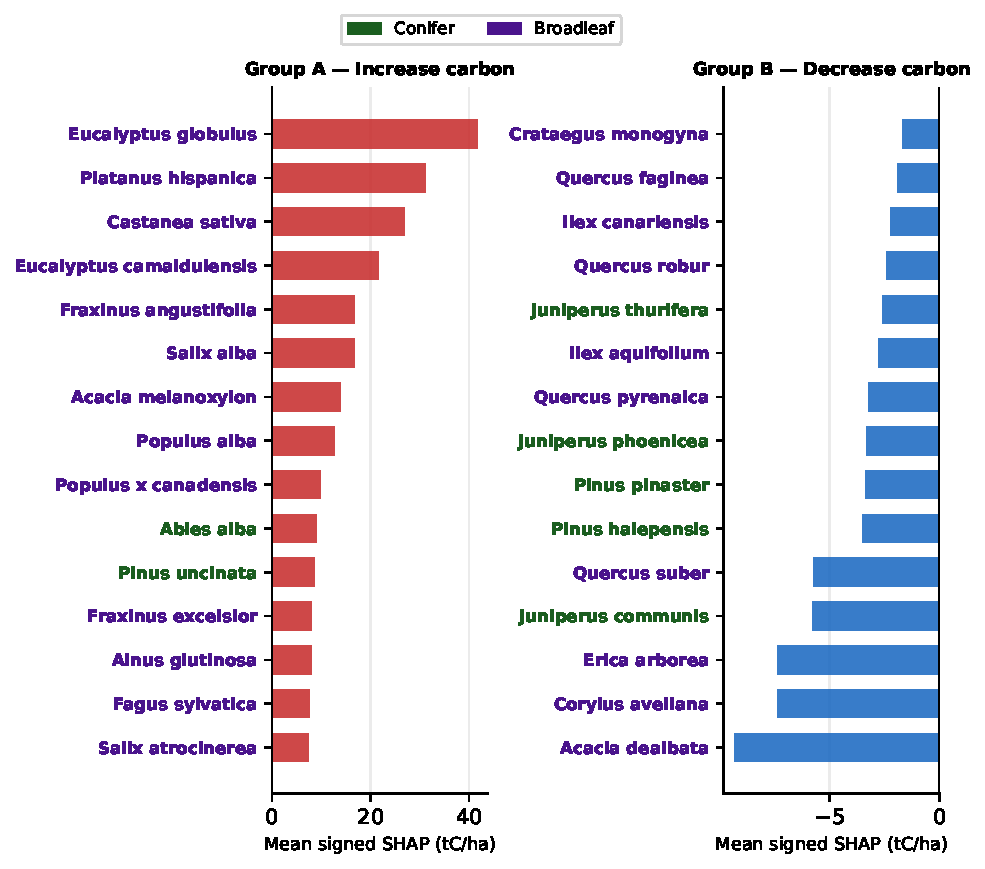
\includegraphics[width=\linewidth]{figuras/09_discusion/species_LightGBM_global.pdf}
      \caption{SHAP analysis for the LightGBM model trained on IFN2 and IFN3 data with target variable \texttt{c4} (tC/ha), focusing on species. A distinction is made between conifer and broadleaf.}
      \label{fig:SHAP_species_LightGBM_global}
\end{figure}

In summary, SHAP analysis not only allows identifying which variables are most relevant for carbon prediction and quantifying their relative importance, but also constitutes an ecological validation tool for the model. The results obtained are consistent with knowledge available in the literature: variables such as tree density, photosynthetic activity, species type or time elapsed between inventories show the expected direction in their SHAP values, indicating that the model has correctly incorporated the input information and that its predictions respond to real ecological processes.



% [Texto de ejemplo. Las figuras enlazadas son reales. El resto están en el repositorio de los modelos. Daltaría comentar el resto de casos.]

% \begin{figure}
%       \centering
%       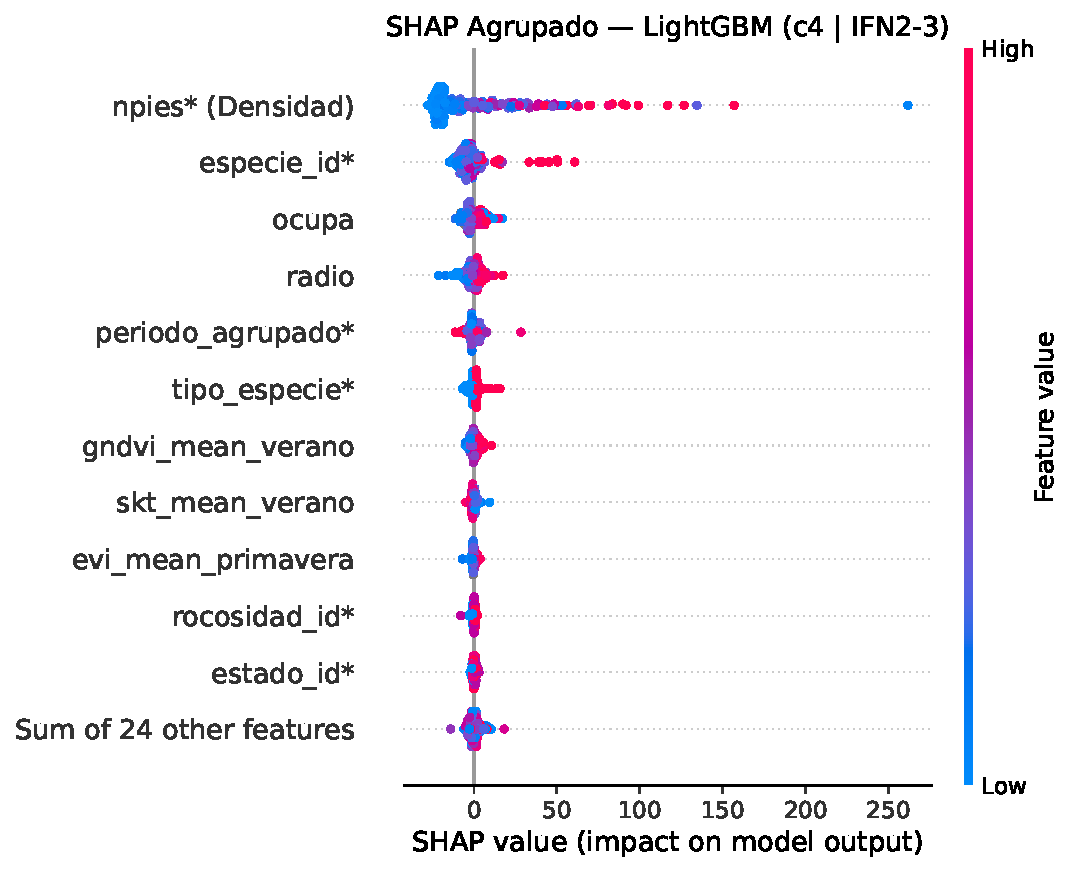
\includegraphics[width=\linewidth]{figuras/09_discusion/beeswarm_grouped_LightGBM.pdf}
%       \caption{Bee swarm plot of LightGBM for variable \texttt{carbono\_bruto4}.}
%       \label{fig:beeswarm_grouped_LightGBM}
% \end{figure}

% \begin{figure}
%       \centering
%       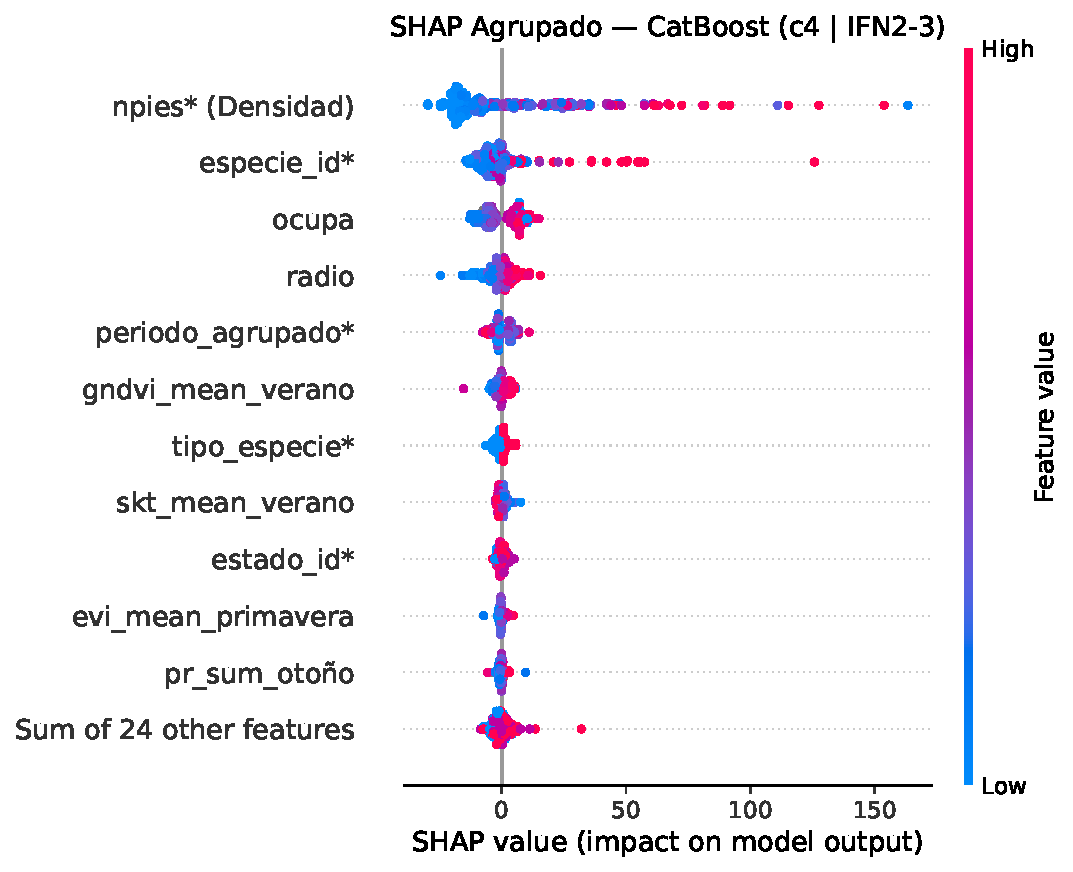
\includegraphics[width=\linewidth]{figuras/09_discusion/beeswarm_grouped_CatBoost.pdf}
%       \caption{Bee swarm plot of CatBoost for variable \texttt{carbono\_bruto4}.}
%       \label{fig:beeswarm_grouped_CatBoost}
% \end{figure}

\vspace{1cm}
\hrule
\vspace{1cm}
